\documentclass[UTF8]{ctexart}
\usepackage{amsmath,amssymb,amsfonts}   % For math symbols and fonts
\usepackage{graphicx}                   % For including images
\usepackage{hyperref}                   % For hyperlinks
\usepackage{cite}                       % For citations
\usepackage[utf8]{inputenc}             % For UTF-8 encoding
% \usepackage[UTF8]{ctex}

\usepackage{algorithm}
\usepackage{algorithmic}

\usepackage{amsthm}
% Define new theorem-like environments
\newtheorem{definition}{Definition}[section]    % Definition environment
\newtheorem{theorem}{Theorem}[section]          % Theorem environment
\newtheorem{exercise}{Exercise}[section]        % Exercise environment


% Title and author info
\title{有限群导引章节翻译}
\author{Zhang Jinrui\thanks{alternative email:jerryzhang40@gmail.com} \\ \texttt{zhangjr1022@mails.jlu.edu.cn}}

\date{20241217}  % Empty date; optional, you can also specify a date here

\begin{document}

\maketitle

\begin{abstract}
    这篇文章翻译了有限群导引第55页-第61页有关群作用
    的基本概念。\cite[有限群导引]{Kurzweil_Stellmacher_2004b}
\end{abstract}

\section{第三章 群作用与共轭}
群作用的概念在有限群的理论中扮演着重要角色。
本章第一节介绍了关于群作用的基本思想和主要结果。
在接下来的两节中,
将利用对陪集的作用证明Sylow定理、
Schur-Zassenhaus定理以及Gaschütz定理。
\subsection{3.1 群作用}
设 $\Omega = \{\alpha, \beta, \dots\}$ 是一个非空有限集。所有对 $\Omega$ 的置换组成的集合 $S_\Omega$ 是一个关于乘法的群,定义如下:
$$
    \alpha^{xy} := (\alpha^x)^y, \quad \alpha \in \Omega, \; x, y \in S_\Omega
$$
$S_\Omega$ 称为 $\Omega$ 上的\textbf{对称群}。我们用 $S_n$ 表示 $\{1, \dots, n\}$ 上的对称群,它是\textbf{阶为 $n$的对称群}。当且仅当 $|\Omega| = n$ 时,有 $S_n \cong S_\Omega$。

当对每一对 $(\alpha, g) \in \Omega \times G$,将元素 $\alpha^g \in \Omega$ 赋予\footnote[1]{虽然在根据定义这里是乘积, 但我们记 $\alpha^g$ 而不是
    $\alpha g$}如下规则:

1. $\mathcal{O}1:$ $ \alpha^1 = \alpha, \; \forall \alpha \in \Omega \;$(其中 $1$ 是单位元 $1_G$);

2. $\mathcal{O}2:$ $ (\alpha^x)^y = \alpha^{xy}, \; \forall x, y \in G, \; \alpha \in \Omega$,

则称群 $G$ 在 $\Omega$ 上作用。

映射
$$
    g^\pi : \Omega \to \Omega, \quad \alpha \mapsto \alpha^g
$$
描述了 $g \in G$ 在 $\Omega$ 上的作用。因为
$$
    (\alpha^g)^{g^{-1}} \overset{\mathcal{O}2}{=} \alpha^{gg^{-1}} = \alpha^1 \overset{\mathcal{O}1}{=} \alpha,
$$
$g^\pi$ 的逆映射是 $(g^{-1})^\pi$,因此 $g^\pi$ 是 $\Omega$ 上的一个置换。由 $O2$ 可知
$$
    \pi: G \to S_\Omega, \quad g \mapsto g^\pi
$$
是一个同态。根据同态基本定理,$G / \ker \pi$ 同构于 $S_\Omega$ 的一个子群,因此也同构于 $S_n$ 的一个子群,其中 $n := |\Omega|$。

反过来,每个同态 $\pi: G \to S_\Omega$ 都给出 $G$ 在 $\Omega$ 上的一个作用(定义为 $\alpha^g := \alpha^{g^\pi}$)。

- 若 $\ker \pi = 1$,称 $G$ 在 $\Omega$ 上作用\textbf{忠实};

- 若 $\ker \pi = G$,称 $G$ 在 $\Omega$ 上作用\textbf{平凡}。

每个 $G$ 在 $\Omega$ 上的作用 $\pi$ 会导出 $G / \ker \pi$ 在 $\Omega$ 上的一个忠实作用:
$$
    \alpha^{(\ker \pi) g} := \alpha^g
$$

下面是一些重要的群作用,在后续章节中会经常遇到。


3.1.1 群G的重要作用


(a) $G$ 通过共轭作用在所有非空子集 $A \subseteq G$ 上:
$$
    A \overset{x}{\mapsto} x^{-1} A x = A^x
$$

(b) $G$ 通过共轭作用在 $G$ 的所有元素 $g \in G$ 上:
$$
    g \overset{x}{\mapsto} x^{-1} g x = g^x
$$

(c) $G$ 通过右乘作用在 $G$ 的一个固定子群 $U$ 的所有右陪集 $Ug$ 上:
$$
    Ug \overset{x}{\mapsto} Ugx
$$



\textbf{证明}
在所有情况下,单位元 $1 = 1_G$ 平凡地作用:这是 $\mathcal{O}1$。结合律保证了 $\mathcal{O}2$。 $\Box$

在 (a) 和 (b) 的情况下,置换 $x^\pi$ 是由 $x$ 引导的内自同构(参见第15页1.3节)。

此外,左乘作用在固定子群 $U$ 的所有左陪集的集合 $\Omega$ 上也给出一个作用 $\pi: G \to S_\Omega$。但在这里,需要定义
$$
    x^\pi : G \to S_\Omega, \quad gU \mapsto x^{-1} gU,
$$
因为 $gU \mapsto xgU$ 不是一个同态(而是一个反同态)\footnote[2]{在3.3中我们将只使用左乘群作用}。


由(c)可以得到:


3.1.2
设 $U$ 是群 $G$ 的一个指数为 $n$ 的子群,则 $G / U_G$ 同构于 $S_n$ 的一个子群\footnote[3]{$U_G=\bigcap_{g\in G} U^g$}。

\textbf{证明}
如 3.1.1(c) 中所述,设 $\Omega$ 是 $U$ 在 $G$ 中的所有右陪集的集合,且 $\pi: G \to S_\Omega$ 是右乘作用。则对于 $x, g \in G$,
$$
    Ugx = Ug \iff gxg^{-1} \in U \iff x \in Ug,
$$
因此
$$
    x^\pi = 1_{S_\Omega} \iff x \in U_G,
$$
即 $U_G = \ker \pi$。 $\Box$



为了处理3.1.1给出的群作用,以下是关于群作用的一些记号和基本性质。这些性质直接由定义推导而来。

设 $G$ 是一个在集合 $\Omega$ 上作用的群,且 $\alpha \in \Omega$。定义
$$
    G_\alpha := \{x \in G \mid \alpha^x = \alpha\},
$$
称 $G_\alpha$ 为 $\alpha$ 在 $G$ 中的稳定子群。若 $x \in G_\alpha$,则称 $x$ 稳定化(固定)$\alpha$。

注意,$G_\alpha$ 是 $G$ 的一个子群,这是由 $\mathcal{O}2$ 保证的。



3.1.3
对于任意 $g \in G, \alpha \in \Omega$,有
$$
    G_\alpha^g = G_{\alpha^g}
$$
\textbf{证明}
$$
    (\alpha^g)^x = \alpha^g \iff (\alpha^{gx}) = \alpha \iff gxg^{-1} \in G_\alpha \iff x \in G_\alpha^g \quad \Box
$$





如果对于任意 $\alpha, \beta \in \Omega$,存在 $x \in G$ 使得 $\alpha^x = \beta$,则称 $\alpha$ 和 $\beta$ 是等价的。由 $\mathcal{O}1$ 和 $\mathcal{O}2$ 可知,这种等价关系确实定义了 $\Omega$ 上的一个等价关系。
与此等价关系对应的等价类称为 $G$ 在 $\Omega$ 上的轨道(或 $G$-轨道)。对于任意 $\alpha \in \Omega$,定义
$$
    \alpha^G := \{\alpha^x \mid x \in G\},
$$
称为包含 $\alpha$ 的轨道。

若 $G$ 在 $\Omega$ 上的作用使得 $\Omega$ 本身是一个轨道(即对所有 $\alpha, \beta \in \Omega$,存在 $x \in G$ 使得 $\alpha^x = \beta$),则称 $G$ 在 $\Omega$ 上作用是\textbf{传递的}。



3.1.4 Frattini引理


假设 $G$ 包含一个在 $\Omega$\footnote[4]{自然的, 我们认为N的作用是G的子群.} 上作用传递的正规子群 $N$,则对任意 $\alpha \in \Omega$,有
$$
    G = G_\alpha N
$$
特别地,若 $N_\alpha = 1$,则 $G_\alpha$ 是 $N$ 在 $G$ 中的一个补群。


\textbf{证明}
令 $\alpha \in \Omega, y \in G$。由于 $N$ 在 $\Omega$ 上作用传递,存在 $x \in N$ 使得 $\alpha^y = \alpha^x$。因此 $\alpha^{yx^{-1}} = \alpha$,即 $yx^{-1} \in G_\alpha$。这表明 $y \in G_\alpha x \subseteq G_\alpha N$。 $\Box$



3.1.5
对于任意 $\alpha \in \Omega$,轨道 $|\alpha^G| = |G : G_\alpha|$。特别地,轨道的长度 $|\alpha^G|$ 是 $|G|$ 的一个因数。


\textbf{证明}
对于任意 $y, x \in G$,
$$
    \alpha^y = \alpha^x \iff \alpha^{yx^{-1}} = \alpha \iff yx^{-1} \in G_\alpha \iff y \in G_\alpha x \quad \Box
$$

由于 $\Omega$ 是 $G$-轨道的并集,显然:


3.1.6
若 $n$ 是一个整数,且 $n$ 整除 $|G : G_\alpha|$ 对于所有 $\alpha \in \Omega$,则 $n$ 也整除 $|\Omega|$。 $\Box$



对于 $U \subseteq G$,定义
$$
    C_\Omega(U) := \{\alpha \in \Omega \mid U \subseteq G_\alpha\},
$$
即 $U$ 在 $\Omega$ 上的所有不动点组成的集合。显然,集合 $\Omega \setminus C_\Omega(G)$ 是所有长度大于 1 的 $G$-轨道的并集。


3.1.7
设 $G$ 是一个 $p$-群,则
$$
    |\Omega| \equiv |C_\Omega(G)| \pmod{p}
$$

\textbf{证明}
对于 $\alpha \in \Omega' := \Omega \setminus C_\Omega(G)$,稳定子群 $G_\alpha$ 是 $G$ 的一个真子群。因此,$p$ 是 $|G : G_\alpha|$ 的一个因数(由 Lagrange 定理),并根据 3.1.6 可得
$$
    |\Omega'| \equiv 0 \pmod{p}
$$
$\Box$


接下来,利用 3.1.3 和 3.1.5 研究 3.1.1 中给出的群作用。

设 $\Omega$ 是 $G$ 的所有非空子集组成的集合,$H \leq G$。则 $H$ 通过共轭作用于 $\Omega$。对于 $A \in \Omega$,集合
$$
    A^x = x^{-1}Ax  ,(x \in H)
$$
是 $H$ 的一个轨道。稳定子群
$$
    N_H(A) := \{x \in H \mid A^x = A\}
$$
称为 $A$ 在 $H$ 中的正规化子。

根据 3.1.5,$|H : N_H(A)|$ 是 $A$ 的 $H$-共轭的数量。

令 $B \in \Omega$。若 $B$ 使得 $B \subseteq N_G(A)$,则称 $B$ 规范化了 $A$。

根据 3.1.1(b),$H$ 通过共轭作用于 $G$ 的所有元素。对于该作用,稳定子群
$$
    C_H(g) := \{x \in H \mid g^x = g\}
$$
称为 $g \in G$ 在 $H$ 中的中心化子。显然,该子群包含所有满足 $xg = gx$ 的元素 $x \in H$。

由 3.1.5 可知,$|H : C_H(g)|$ 是 $g$ 的 $H$-共轭的数量。

对于 $G$ 的非空子集 $A$,定义
$$
    C_H(A) := \bigcap_{g \in A} C_H(g),
$$
称为 $A$ 在 $H$ 中的中心化子。因此,$C_H(A)$ 包含所有与 $A$ 的每个元素对易的 $H$ 中的元素。例如,当且仅当 $A \subseteq Z(G)$ 时,有 $C_G(A) = G$。如果 $B \subseteq C_G(A)$(等价于 $[A, B] = 1$,参见第25页),则称 $B$ 中心化了 $A$。

由 3.1.3 可得,对于任意 $x \in G$,
$$
    N_G(A)^x = N_G(A^x), \quad C_G(A)^x = C_G(A^x)
$$
更一般地,
$$
    N_H(A)^x = N_{H^x}(A^x), \quad C_H(A)^x = C_{H^x}(A^x)
$$

在 $H = G$ 的情况下,$G$ 的轨道 $g^G$ 称为 $g \in G$ 的共轭类,并且
$$
    |g^G| = |G : C_G(g)|
$$

群 $Z(G)$ 包含所有共轭类长度为 1 的元素,即仅与自身共轭的元素。

由于 $G$ 是其共轭类的并集,这些类是通过共轭作用定义的 $G$-轨道,因此有:


3.1.8 共轭类方程
设 $K_1, \dots, K_h$ 是长度大于 1 的 $G$ 的共轭类,令 $a_i \in K_i$($i = 1, \dots, h$)则
$$
    |G| = |Z(G)| + \sum_{i=1}^h |G : C_G(a_i)| \quad \Box
$$


注意到:

3.1.9
设 $U$ 是 $G$ 的一个子群,则 $N_G(U)$ 是 $U$ 在 $G$ 中的最大正规化子。映射
$$
    \varphi : N_G(U) \to \text{Aut}(U), \quad x \mapsto (u \mapsto u^x)
$$
是一个同态,其核为 $C_G(U)$。特别地,$N_G(U)/C_G(U)$ 同构于\footnote[5]{13页1.2.5同态定理} $\text{Aut}(U)$ 的一个子群。 $\Box$


我们通过两个从3.1.7带出的p-子群和p-群的重要性质来结束此章节。

3.1.10
设 $P$ 是 $G$ 的一个 $p$-子群,且 $p$ 整除 $|G : P|$。则
$$
    P < N_G(P)
$$

\textbf{证明}
根据 3.1.1(c),$P$ 通过右乘作用于右陪集 $Pg, g \in G$ 的集合 $\Omega$,且
$$
    |\Omega| = |G : P| \equiv 0 \pmod{p}
$$
由 3.1.7(将 $P$ 替代 $G$),有
$$
    |C_\Omega(P)| \equiv |\Omega| \equiv 0 \pmod{p}
$$
此外,$P \in C_\Omega(P)$,因此 $C_\Omega(P) \neq \varnothing$。存在 $Pg \in C_\Omega(P)$,且 $P \neq Pg$。这意味着 $g \notin P$,且 $PgP = Pg$。因此 $gPg^{-1} = P$,即 $g \in N_G(P) \setminus P$。 $\Box$


3.1.11
设 $P$ 是一个 $p$-群,$N \neq 1$ 是 $P$ 的一个正规子群,则
$$
    Z(P) \cap N \neq 1
$$
特别地,$Z(P) \neq 1$

\textbf{证明}
$P$ 通过共轭作用于 $\Omega := N$,且
$$
    C_\Omega(P) = Z(P) \cap N
$$
由于 $N$ 是一个 $p$-群,由 3.1.7 可得
$$
    |C_\Omega(P)| \equiv |\Omega| \equiv 0 \pmod{p}
$$
由于 $1 \in C_\Omega(P)$,有 $|C_\Omega(P)| \geq p$。 $\Box$






% \section{Motivation of Separation Axioms}
% The basic Axioms of topology only described the relationship of the
% opensets, the opensets captured the geometry structure in the point set.
% but it some of the coarse topology dose not have a much resonable
% behavior, such as the indiscrete topology, even the const sequence
% could converge to any point in the base set. this is because the
% topology is so coarse that we only have two opensets that is $\{\phi, X\}$
% so all the structure we care is crushed together in this topology.

% The Separation Axioms served as patched to the basic Axioms of topology
% to make sure we are deal with some topology space with some familiar
% behaviors. This is the motivation and mean of Introduction these
% Axioms patches.\cite[script1]{MAT327topology1script}

% \section{All the Axioms}
% \subsection{Definition of Separation Axioms}
% First lets see three basic separation concepts,
% that is Hausdorff, regular and normal.
% Figure\ref{fig:regular} has well illustrated the
% idea.
% \begin{definition}[regular]
%     A topological space X is a regular space if,
%     given any closed set F and any point x that
%     does not belong to F, there exists a neighbourhood
%     U of x and a neighbourhood V of F
%     that are disjoint. Concisely put,
%     it must be possible to separate x and F
%     with disjoint neighborhoods.
%     \cite[Reglarspace]{Reglarspace}
%     Figure\ref{fig:regular}
% \end{definition}
% \begin{definition}[normal]
%     A topological space X is a normal space if, given
%     any disjoint closed sets E and F, there are
%     neighbourhoods U of E and V of F that are also
%     disjoint. More intuitively, this condition says
%     that E and F can be separated by neighbourhoods.
%     \cite[Normal]{Normal}
%     % Figure\ref{fig:regular}
% \end{definition}
% \begin{definition}[closed neighborhoods separation]
%     We say that x and y can be separated by closed
%     neighborhoods if there exists a closed neighborhood
%     U of x and a closed neighborhood V of y such that U
%     and V are disjoint $(U \cap V = \emptyset)$.
%     (Note that a "closed neighborhood of x" is
%     a closed set that contains an open set
%     containing x.)
%     \cite[UandcHs]{UandcHs}
% \end{definition}
% Another important concept is completeness.
% The prefix "completely" add ahead the
% Hausdorff, regular and normal neams the
% corresponding two object can be separate
% by functions.
% \begin{definition}[continuous separation]
%     We say that x and y can be separated by a function
%     if there exists a continuous function
%     $f:X \to [0,1]$ (the unit interval) with
%     $f(x) = 0$ and $f(y) = 1$.
%     \cite[UandcHs]{UandcHs}
% \end{definition}
% \begin{definition}[set separate by function]
%     We say that two sets X and Y can
%     be separated by a function
%     if there exists a continuous function
%     $f:X \to [0,1]$ (the unit interval) with
%     $f\vert _{X} = 0$ and $\vert _{Y} = 1$.
%     \cite[UandcHs]{UandcHs}
% \end{definition}
% \begin{definition}[completely regular]
%     A topological space
%     X is called completely regular if points can be
%     separated from closed sets via (bounded) continuous real-valued functions. In technical terms this means: for any closed set
%     ${\displaystyle A\subseteq X}$ and any point,
%     ${\displaystyle x\in X\setminus A,}$ there
%     exists a real-valued continuous function
%     ${\displaystyle f:X\to \mathbb {R} }$ such that
%     ${\displaystyle f(x)=1}$ and
%     ${\displaystyle f\vert _{A}=0.}$ \
%     (Equivalently one can choose any two values
%     instead of
%     ${\displaystyle 0}$ and
%     ${\displaystyle 1}$ and even require that
%     ${\displaystyle f}$ be a bounded function.)
%     \cite[Tychonoff]{Tychonoff}
% \end{definition}
% The following part is all the $T$ Axioms.
% \begin{definition}[$T_0$]
%     A topological space $(X, \mathcal{T})$ is said to be $T_0$ (or much less commonly said to
%     be a Kolmogorov space), if for any pair of distinct points $x, y \in X$ there is an open set U that
%     contains one of them and not the other.
%     \cite[script5]{MAT327topology5script}
% \end{definition}
% \begin{definition}[$T_1$]
%     A topological space $(X, \mathcal{T})$ is said to be $T_1$ (or much less commonly said to be
%     a Fr\'echet space) if for any pair of distinct points $x, y \in X$, there exist open sets U and V such
%     that U contains x but not y, and V contains y but not x.
%     \cite[script5]{MAT327topology5script}
% \end{definition}
% \begin{definition}[$T_2$]
%     A topological space $(X, \mathcal{T})$ is said to be $T_2$, or more commonly said to be
%     a Hausdorff space, if for every pair of distinct points $x, y \in X$, there exist disjoint open sets $U$
%     and $V$ such that $x \in U$ and $y \in V$.
%     \cite[script5]{MAT327topology5script}
% \end{definition}
% \begin{theorem}
%     Let $(X, \mathcal{T})$ be a Hausdorff space. Then every sequence in $X$
%     converges to at most one point.
%     \cite[script5]{MAT327topology5script}
% \end{theorem}
% $Proof.$ Suppose $X$ is Hausdorff and let ${x_n}$ be a sequence in $X$. Suppose $x_n \to x$ and $y \not= x$.
% Then there are disjoint open sets $U$ and $V$ such that $x \in U$ and $y \in V$ . By definition of
% convergence, some tail of the sequence is in the set U. But then that tail (and therefore all tails
% of the sequence) is disjoint from $V$ , meaning $x_n \not\to y$.\cite[script5]{MAT327topology5script}
% \begin{definition}[$T_{2\frac{1}{2}}$]
%     A Urysohn space, also called a $T_{2\frac{1}{2}}$
%     space, is a space in which any two distinct points
%     can be separated by closed neighborhoods.
%     \cite[UandcHs]{UandcHs}
% \end{definition}
% \begin{definition}[completely $T_2$]
%     A completely Hausdorff space, or completely $T_2$,
%     or functionally
%     Hausdorff space, is a space in which any two
%     distinct points can be separated by a continuous
%     function.
%     \cite[UandcHs]{UandcHs}
% \end{definition}
% \begin{definition}[$T_3$]
%     A $T_3$ space or regular Hausdorff space is a
%     topological space that is both regular and a
%     Hausdorff space.
%     \cite[Reglarspace]{Reglarspace}
% \end{definition}
% \begin{definition}[$T_{3\frac{1}{2}}$]
%     A topological space is called a
%     Tychonoff space (alternatively:
%     $T_{3\frac{1}{2}}$ space, or $T_\pi$ space,
%     or completely
%     $T_3$ space) if it is a
%     completely regular Hausdorff space.
%     \cite[Tychonoff]{Tychonoff}
% \end{definition}
% \begin{definition}[$T_4$]
%     A T4 space is a $T_1$ space X that is normal;
%     this is equivalent to X being normal and
%     Hausdorff.
%     \cite[Tychonoff]{Tychonoff}
% \end{definition}
% \begin{definition}[$T_5$]
%     A $T_5$ space, or completely $T_4$ space,
%     is a completely normal $T_1$ space X,
%     which implies that X is Hausdorff;
%     equivalently, every subspace of X
%     must be a $T_4$ space.
%     \cite[Tychonoff]{Tychonoff}
% \end{definition}
% \begin{definition}[$T_6$]
%     A $T_6$ space, or perfectly $T_4$ space,
%     is a perfectly normal Hausdorff space.
%     \cite[Tychonoff]{Tychonoff}
% \end{definition}

% \subsection{Some properties}
% \begin{theorem}[$T_0$ hereditary]
%     If a space is $T_0$ then its subspace is
%     also $T_0$
% \end{theorem}
% $Proof.$ The subspace presere the open sets
% of the original space. The definition of the
% $T_0$ space only contains the definition
% of the open sets.

% Suppose $x,y\in E\subset X$ then
% $\exists U\in \mathcal{T}$
% that $x\in U, y \not\in U$
% then $U_E = E \cap U \in \mathcal{T}_E$
% that $x\in U_E, y \not\in U_E$

% \begin{theorem}[$T_0$ productspace]
%     If a space is $T_0$ then its productspace is
%     also $T_0$
% \end{theorem}
% $Proof.$ The productspace also can
% presere the open sets
% of the original space.

% Suppose $(X,\mathcal{T}_X),(Y,\mathcal{T}_Y)$ are
% $T_0$ space.
% then the product space
% $(P,\mathcal{T}_P)
%     =
%     (X\times Y, \mathcal{T}_X\times\mathcal{T}_Y)$
% if two points
% $(x,y)\not=(x',y')\in P$
% then there at least one coordinate are distinct
% Suppose $x\not=x'$ then
% $\exists U\in \mathcal{T_X}$
% that $x\in U, x' \not\in U$
% then
% $\exists U_P=U\times Y\in \mathcal{T_P}$
% that
% that $x\in U_P, x' \not\in U_P$

% For the continuous image $X\to Y$.
% We can just let $(Y,\mathcal{T}_{trivial})$
% then any Separation Axioms would not presere
% in the image $f(X)\subset Y$

% \subsection{Examples and counterExamples}
% Spaces that are not $T_0$

% A set with more than one element, with the trivial topology. No points are distinguishable.

% The set R2 where the open sets are the Cartesian product of an open set in R and R itself, i.e., the product topology of R with the usual topology and R with the trivial topology; points (a,b) and (a,c) are not distinguishable.

% The space of all measurable functions f from the real line R to the complex plane C such that the Lebesgue integral
% ${\displaystyle \left(\int _{\mathbb {R} }|f(x)|^{2}\,dx\right)^{\frac {1}{2}}<\infty }$. Two functions which are equal almost everywhere are indistinguishable. See also below.

% Spaces that are $T_0$ but not $T_1$

% The Zariski topology on Spec(R), the prime spectrum of a commutative ring R, is always $T_0$ but generally not $T_1$. The non-closed points correspond to prime ideals which are not maximal. They are important to the understanding of schemes.

% The particular point topology on any set with at least two elements is $T_0$ but not $T_1$ since the particular point is not closed (its closure is the whole space). An important special case is the Sierpiński space which is the particular point topology on the set {0,1}.

% The excluded point topology on any set with at least two elements is $T_0$ but not $T_1$. The only closed point is the excluded point.

% The Alexandrov topology on a partially ordered set is $T_0$ but will not be $T_1$ unless the order is discrete (agrees with equality). Every finite $T_0$ space is of this type. This also includes the particular point and excluded point topologies as special cases.

% The right order topology on a totally ordered set is a related example.

% The overlapping interval topology is similar to the particular point topology since every non-empty open set includes 0.

% Quite generally, a topological space X will be $T_0$ if and only if the specialization preorder on X is a partial order. However, X will be $T_1$ if and only if the order is discrete (i.e. agrees with equality). So a space will be $T_0$ but not $T_1$ if and only if the specialization preorder on X is a non-discrete partial order.
% \subsection{Relationship between Separation Axioms}
% $
%     T_6
%     \Rightarrow T_5
%     \Rightarrow T_4
%     \Rightarrow T_{3\frac{1}{2}}
%     \Rightarrow T_3
%     \Rightarrow T_{2\frac{1}{2}}
%     \Rightarrow T_2
%     \Rightarrow T_1
%     \Rightarrow T_0
% $

% Each implication is strict

% \section{Results}
% \subsection{first approach}
% Train the model on a pure $sin(x)$ and try to
% get a result that satisfies the initial condition with
% $U^{t}_0=0.5$ and $U_0=0.0$ to which the exact solution is $0.5*sin(x)$ would. The result is shown in Figure\ref{fig:fig1}.
% \subsection{approach with linear assumption}
% Train the model on a pure $sin(x)$ and try to
% get a result that satisfies the initial condition with
% $U^{t}_0=0.5$ and $U_0=0.5$ in which the exact solution is $\frac{\sqrt{2}}{2}*sin(x+\frac{\pi}{4})$ would be
% required output. The result is shown in Figure\ref{fig:fig2}.
% \subsection{approach augmentation}
% Train the model on a 2D circle and try to
% get a result of $x^\delta=y^\delta(\rho)=[cos(\rho),sin(\rho)]$,
% and the corresponding differential equation is
% $\frac{\partial^2 y_\delta}{{\partial \rho}^2}+y_\delta=0$
% Result of the latent space structure shows in Figures\ref{fig:fig3} and Figure\ref{fig:fig4}, with the
% numerical result $0.7360\frac{\partial^2 y_\delta}{{\partial \rho}^2}-0.0328\frac{\partial y_\delta}{{\partial \rho}}+  0.6761y_\delta=0$.

% \begin{figure}[h!]
%     \centering
%     \includegraphics[width=0.45\textwidth]{figde3/draw_2D__GeneredData.png}
%     \includegraphics[width=0.5\textwidth]{figde3/draw_2D__GeneredEqu.png}
%     \caption{generated data using the PINN to get $0.5*sin(x)$}
% \end{figure}
% \begin{figure}[ht!]
%     \centering
%     \begin{minipage}{0.45\textwidth}
%         \centering
%         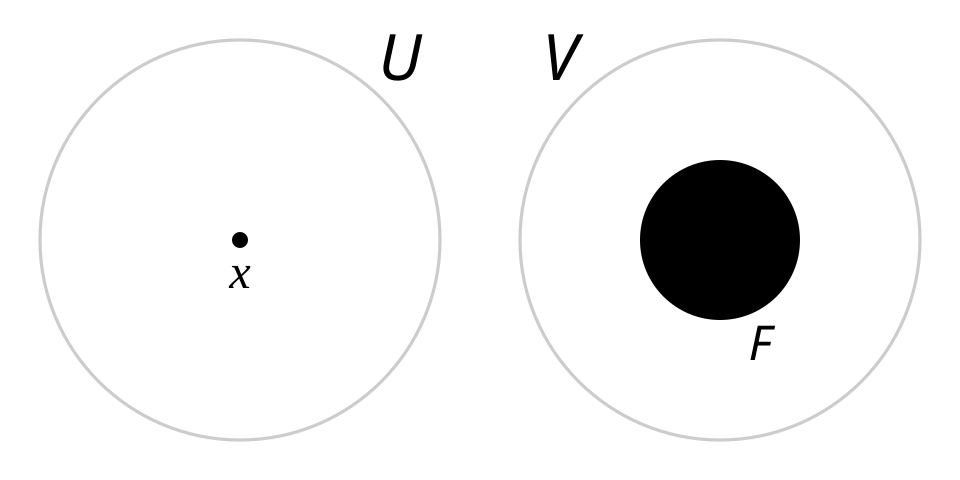
\includegraphics[width=0.9\textwidth]{images/Regular_space.svg.png} % first figure itself
%         \caption{regular}
%         \label{fig:regular}
%     \end{minipage}\hfill
%     \begin{minipage}{0.45\textwidth}
%         \centering
%         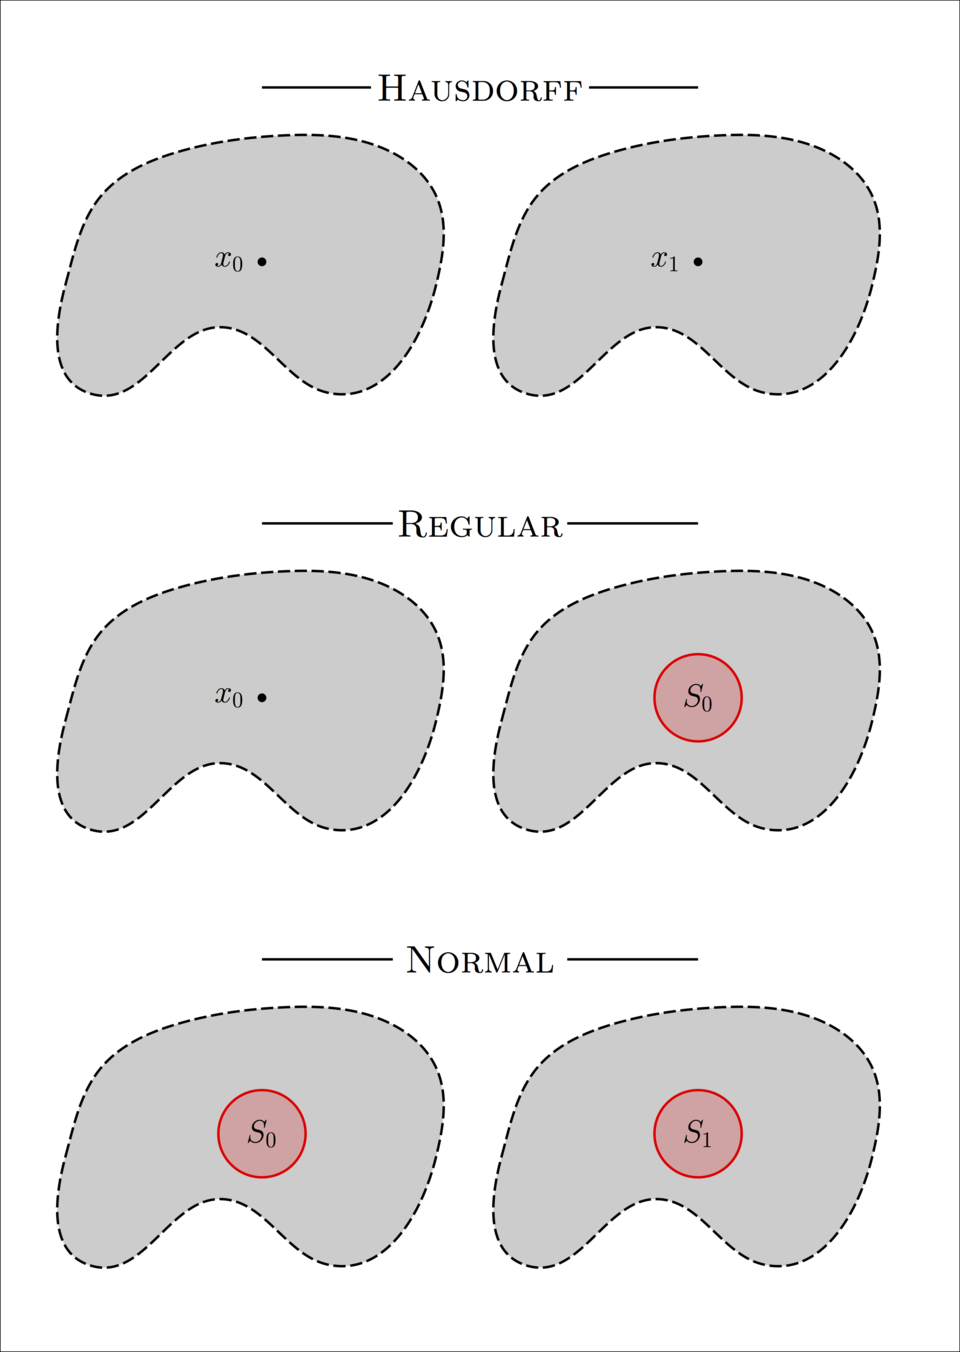
\includegraphics[width=0.9\textwidth]{images/960px-Hausdorff_regular_normal_space_diagram.png} % first figure itself
%         \caption{regular, normal and Hausdorff}
%         \label{fig:normalregHous}
%     \end{minipage}
% \end{figure}
% \begin{figure}[ht!]
%     \centering
%     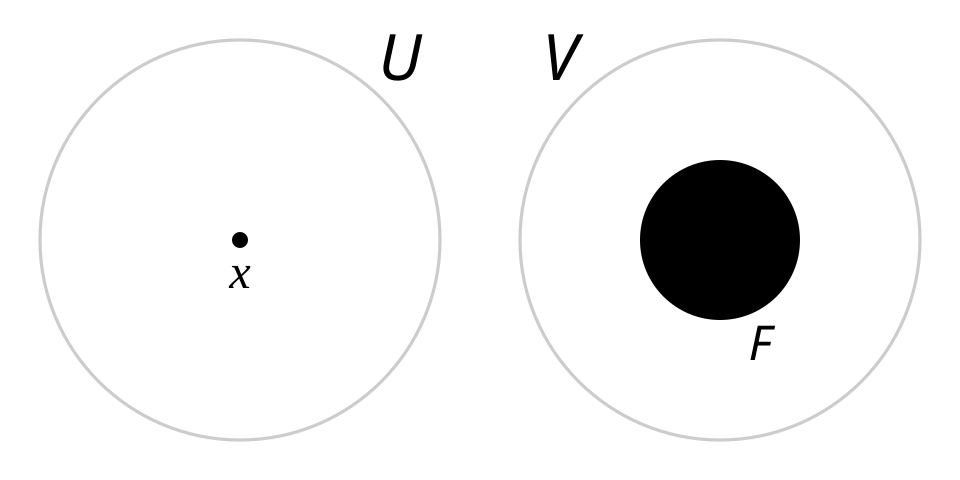
\includegraphics[width=0.9\textwidth]{images/Regular_space.svg.png} % first figure itself
%     \caption{regular}
%     \label{fig:regular}
% \end{figure}
% \begin{figure}[ht!]
%     \centering
%     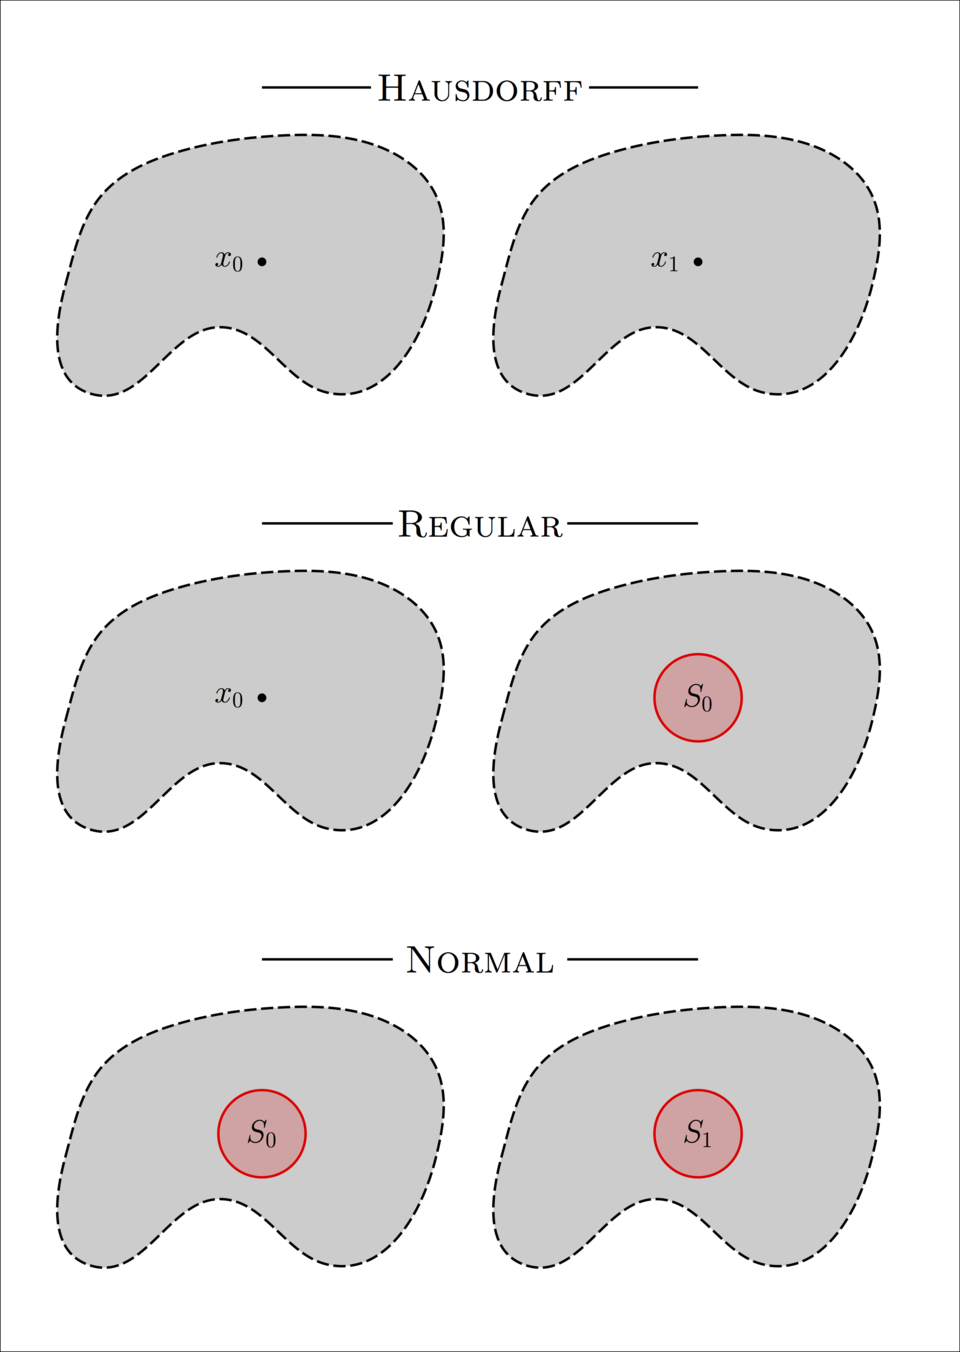
\includegraphics[width=0.9\textwidth]{images/960px-Hausdorff_regular_normal_space_diagram.png} % first figure itself
%     \caption{regular, normal and Hausdorff}
%     \label{fig:normalregHous}
% \end{figure}
% \begin{figure}[ht!]
%     \centering
%     \begin{minipage}{0.45\textwidth}
%         \centering
%         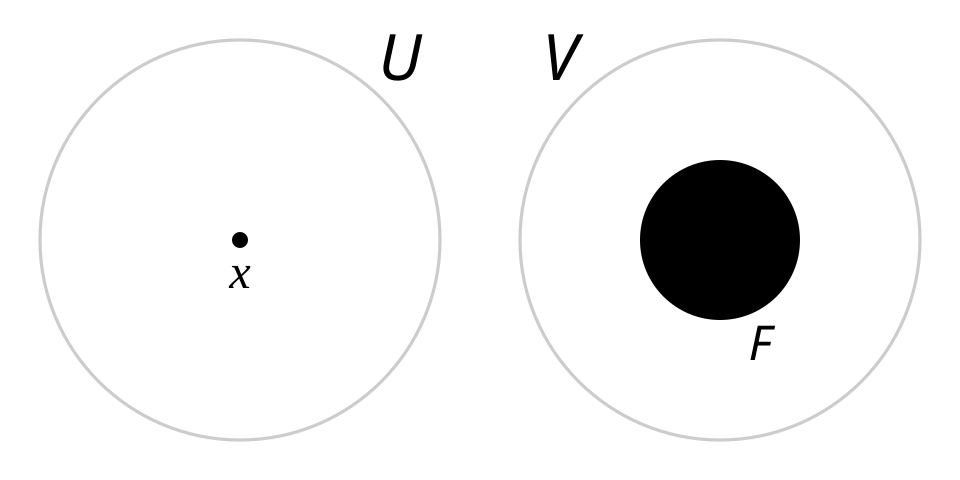
\includegraphics[width=0.9\textwidth]{images/Regular_space.svg.png} % first figure itself
%         \caption{regular}
%         \label{fig:fig1}
%     \end{minipage}\hfill
% \end{figure}
% \begin{figure}[ht!]
%     \centering
%     \begin{minipage}{0.45\textwidth}
%         \centering
%         \includegraphics[width=0.9\textwidth]{figLinearSine1_cbf0039b/draw_2D__GeneredData.png} % first figure itself
%         \caption{$\frac{\sqrt{2}}{2}*sin(x+\frac{\pi}{4})$}
%         \label{fig:fig2}
%     \end{minipage}\hfill
%     \begin{minipage}{0.45\textwidth}
%         \centering
%         \includegraphics[width=0.9\textwidth]{figLinearSine1_cbf0039b/draw_2D__GeneredEqu.png} % second figure itself
%         \caption{$f$ errors}
%     \end{minipage}
% \end{figure}
% \begin{figure}[ht!]
%     \centering
%     \begin{minipage}{0.45\textwidth}
%         \centering
%         \includegraphics[width=0.9\textwidth]{figAugWithP/draw_3D__latentPlot0.png} % first figure itself
%         \caption{first component latent space of $y^\delta(\rho)$}
%         \label{fig:fig3}
%     \end{minipage}\hfill
%     \begin{minipage}{0.45\textwidth}
%         \centering
%         \includegraphics[width=0.9\textwidth]{figAugWithP/draw_3D__latentPlot1.png} % second figure itself
%         \caption{second component latent space of $y^\delta(\rho)$}
%     \end{minipage}
% \end{figure}
% \begin{figure}[ht!]
%     \centering
%     \begin{minipage}{0.45\textwidth}
%         \centering
%         \includegraphics[width=0.9\textwidth]{figAugWithP/draw_2D__circleData.png} % first figure itself
%         \caption{original data $x_\delta$}
%         \label{fig:fig4}
%     \end{minipage}\hfill
%     \begin{minipage}{0.45\textwidth}
%         \centering
%         \includegraphics[width=0.9\textwidth]{figAugWithP/draw_2D__circleGeneInTask.png} % second figure itself
%         \caption{regenerate data $y_\delta$}
%     \end{minipage}
% \end{figure}


% \begin{thebibliography}{99}
%     % Use \bibitem to reference your sources. Example:
%     \bibitem{example-ref} Author Name, \textit{Title of the Paper}, Journal, Year.
% \end{thebibliography}
\bibliographystyle{plain}  % or another style like unsrt, IEEEtran, etc.
\bibliography{references}  % references.bib is the file name

\end{document}
